% main.tex
\documentclass[10pt,a4paper]{ctexbook}
\usepackage{makeidx} % 调用 makeidx 宏包,用来处理索引
\usepackage{tabto}
\usepackage{tikz}                   % 绘制图形
\usepackage{tikz-3dplot}            % 绘制三维坐标系,坐标变换
\usepackage{siunitx}
\usepackage{indentfirst}
\usepackage{amsmath}
\usepackage{geometry}
\usepackage{pgfplots}
\usepackage{tcolorbox}

\usepackage{tcolorbox}
\usepackage{colortbl}
\usepackage{geometry}


\usepackage{physics}
\usepackage{amsmath}
\usepackage{tikz}
\usepackage{mathdots}
\usepackage{yhmath}
\usepackage{cancel}
\usepackage{color}
\usepackage{siunitx}
\usepackage{array}
\usepackage{multirow}
\usepackage{amssymb}
\usepackage{gensymb}
\usepackage{tabularx}
\usepackage{extarrows}
\usepackage{booktabs}
\usetikzlibrary{fadings}
\usetikzlibrary{patterns}
\usetikzlibrary{shadows.blur}
\usetikzlibrary{shapes}


\usepackage{xparse}


\usepackage{newtxtext}
\usepackage{geometry}
\usepackage{lipsum} % 该宏包是通过 \lipsum 命令生成一段本文,正式使用时不需要引用该宏包
\usepackage[dvipsnames,svgnames]{xcolor}
\usepackage[strict]{changepage} % 提供一个 adjustwidth 环境
\usepackage{framed} % 实现方框效果

\def\TeacherName{郑老师}

% environment derived from framed.sty: see leftbar environment definition
\definecolor{formalshade}{rgb}{0.95,0.95,1} % 文本框颜色
% ------------------******-------------------
% 注意行末需要把空格注释掉,不然画出来的方框会有空白竖线
\newenvironment{formal}{%
\def\FrameCommand{%
\hspace{1pt}%
{\color{DarkBlue}\vrule width 2pt}%
{\color{formalshade}\vrule width 4pt}%
\colorbox{formalshade}%
}%
\MakeFramed{\advance\hsize-\width\FrameRestore}%
\noindent\hspace{-4.55pt}% disable indenting first paragraph
\begin{adjustwidth}{}{7pt}%
\vspace{2pt}\vspace{2pt}%
}
{%
\vspace{2pt}\end{adjustwidth}\endMakeFramed%
}
% ------------------******-------------------


\newcommand{\classinfo}[4]{
\begin{center}
    \begin{tabular}{ | m{5em}<{\centering} | m{4em}<{\centering}| m{4em}<{\centering} | m{4em}<{\centering} | m{5em}<{\centering} | m{5em}<{\centering} | m{4em}<{\centering} | m{5em}<{\centering} | } 
    \hline
    教师姓名& \TeacherName & 学生姓名&   & 等级& #1 & 上课时间 & \\ 
    \hline
    学\quad\quad 科& 高中数学 & 课题名称 &  \multicolumn{5}{c|}{#2} \\ 
    \hline
    教学目标 & \multicolumn{7}{l|}{#3} \\ 
    \hline
    教学重难点 & \multicolumn{7}{l|}{#4} \\ 
    \hline
    \end{tabular}
 \end{center}
}



\newif\ifprint

\newcommand{\tiankong}[1]{\ \underline{
\ifprint
\ #1
\else
\hspace*{5em}
\fi}}

\newif\ifjiexi
\NewDocumentEnvironment{jiexi}{ +b }{
\ifjiexi
\par
{\bfseries 解析}\, #1
\else
{\vspace{2cm}}
\fi
}{\par}

\newif\ifshowanswer
\showanswerfalse %答案控制看这里

\ifshowanswer
\printtrue
\jiexitrue
\else
\printfalse
\jiexifalse
\fi 


\geometry{a4paper,hmargin=0.8in,vmargin=0.7in} %设置上下左右边距

\title{沪教版高中数学讲义} 
\author{ 郑振宇\thanks{邮箱:coyatzheng@gmail.com}}
\date{\today}


\begin{document}
\newtheorem{problem}{例}[section]
\setlength{\parindent}{0em}


\maketitle



\chapter{集合与逻辑}
ssss
\chapter{等式和不等式}

\section{等式的性质与方程的解集}
\begin{enumerate}
    \item 等式的性质
    \begin{enumerate}
        \item 传递性 \NumTabs{16} 设$a,b$均为实数,如果$a=b$,且$b=c$,那么$a=c$ 
        \item 加法性质 \NumTabs{16} 设$a,b$均为实数,那么$a+c=b+c$ 
        \item 乘法性质 \NumTabs{16} 设$a,b$均为实数,那么$ac=bc$ 
    \end{enumerate}
    \item 方程的解集 \quad  含有未知数的等式称为方程.使得方程两端相等的未知数的值,称为方程的解或者方程的根。
    以方程的解为元素所构成的集合称为方程的解集。
\end{enumerate}

\section{一元二次方程的解集及根与系数的关系}

1、概念:形如 $ax^2+bx+c,(a \ne 0)$ 的方程为一元二次方程;\par
2、配方法:对一元二次方程进行配方得到方程:$\displaystyle(x + \frac{b}{2a})^2 = \frac{b^2-4ac}{4a^2} $ \par
3、判别式$\Delta$ \par
从配方之后的方程可以看出:原方程有没有解,取决于代数式$ b^2-4ac $的正负;基于$ b^2-4ac $的重要性,令称为该一元二次方程的判别式,它决定了一元二次方程解的个数问题;\par
(1)若$\Delta > 0$,原方程有两个不等的实数根,这两个根是$\displaystyle x_1 = \frac{-b+\sqrt{b^2-4ac}}{2a} , x_2 = \frac{-b-\sqrt{b^2-4ac}}{2a}$;\par
(2)若$\Delta = 0$,原方程有两个相等的实数根,$\displaystyle x_1 = x_2 = -\frac{b}{2a}$;\par
(3)若$\Delta < 0$,原方程没有实根;\par
4、韦达定理\par
当上述一元二次方程有实数解时,$\displaystyle x_1 = \frac{-b+\sqrt{b^2-4ac}}{2a} , x_2 = \frac{-b-\sqrt{b^2-4ac}}{2a}$ \par
则:$$ x_1+x_2=\frac{-b+\sqrt{\Delta}}{2a}+\frac{-b-\sqrt{\Delta}}{2a}=-\frac{b}{a}$$
$$ x_1 \cdot x_2=\frac{-b+\sqrt{b^2-4ac}}{2a} \cdot \frac{-b-\sqrt{b^2-4ac}}{2a}=  \frac{c}{a}$$

注意:在现在所学范围下,使用韦达定理时,需判别$\Delta = b^2-4ac \ge 0 $. \par
特别的:
$$x_1^2+x_2^2 = (x_1+x_2)^2-2x_1x_2 \qquad \qquad \frac{1}{x_1}+\frac{1}{x_2} = \frac{x_1+x_2}{x_1x_2}$$
$$(x_1-x_2)^2 = (x_1+x_2)^2-4x_1x_2 \qquad \qquad | x_1-x_2 | = \sqrt{(x_1+x_2)^2-4x_1x_2}$$
{一元二次方程的两根之差的绝对值$\displaystyle | x_1-x_2 | =  \frac{\sqrt{\Delta}}{|a|}$\par}


\clearpage
\section{第6课\quad 不等式的求解1}
考点一、一元一次不等式组求解\par
(同大取大,同小取小,大小交叉中间找,大大小小没有解)

考点二、一元二次不等式求解\par
(方程的根-函数草图-观察求解)

考点三、一元二次方程根的分布\par
一元二次方程$ax^2+bx+c=0\quad (a,b,c \in R,a>0)$两实根为$x_1,x_2 \Leftrightarrow$函数$f(x)=ax^2+bx+c$与$x$轴交点为$(x_1,0),(x_2,0)$

(1)\quad $\displaystyle x_{1}>0,x_2>0 \Leftrightarrow \left\{
\begin{aligned}
\Delta \ge 0 \\
x_1+x_2>0 \\
x_1 \cdot x_2 > 0
\end{aligned}
\right. 
\Leftrightarrow 
\left\{
\begin{aligned}
\Delta \ge 0 \\
-\frac{b}{2a}>0 \\
f(0) > 0
\end{aligned}
\right. 
$   其中$\displaystyle \Delta=b^2-4ac,x_1+x_2=-\frac{b}{a},x_1 \cdot x_2=\frac{c}{a}$;\par

(2)\quad $\displaystyle x_{1}<0,x_2<0 \Leftrightarrow \left\{
\begin{aligned}
\Delta \ge 0 \\
x_1+x_2<0 \\
x_1 \cdot x_2 > 0
\end{aligned}
\right. 
\Leftrightarrow 
\left\{
\begin{aligned}
\Delta \ge 0 \\
-\frac{b}{2a}<0 \\
f(0) > 0
\end{aligned}
\right. 
$ ;\par
(3)\quad $\displaystyle x_{1}>0,x_2<0 \Leftrightarrow \left\{
\begin{aligned}
\Delta > 0 \\
x_1 \cdot x_2 < 0
\end{aligned}
\right. 
\Leftrightarrow 
f(0) < 0
$ ;\par
(4)\quad $\displaystyle x_{1}>m,x_2>m \Leftrightarrow \left\{
\begin{aligned}
\Delta \ge 0 \\
(x_1-m)+(x_2-m)>0 \\
(x_1-m)\cdot(x_2-m) > 0
\end{aligned}
\right. 
\Leftrightarrow 
\left\{
\begin{aligned}
\Delta \ge 0 \\
-\frac{b}{2a}>0 \\
f(m) > 0
\end{aligned} 
\right. 
$\par
(5)\quad $\displaystyle x_{1}<m<x_2 \Leftrightarrow \left\{
\begin{aligned}
\Delta > 0 \\
(x_1-m)\cdot(x_2-m) < 0
\end{aligned}
\right. 
\Leftrightarrow 
f(m) < 0
$\par
(6)\quad $\displaystyle x_{1},<x_2 \in(m,n) \Leftrightarrow \left\{
\begin{aligned}
\Delta \ge 0 \\
m<-\frac{b}{2a}<n \\
f(m) > 0\\
f(n) > 0
\end{aligned}
\right. 
$

\clearpage
\section{第7课\quad 不等式的求解2}

\begin{formal}
    {\large \textbf{知识点一、分式不等式的解法}}
\end{formal}
1、定义:型如$\displaystyle \frac{f(x)}{\varphi(x)}>0$或$\displaystyle \frac{f(x)}{\varphi(x)}<0$,(其中$f(x),\varphi(x)$为整式且$\varphi(x)\ne 0$)的不等式称为分式不等式.\par
2、解法\par
\begin{enumerate}
    \item 化分式不等式一边为零.
    \item 应用同号相乘(除)得正,异号相乘(除)得负,转化为同解不等式组解之
    \item 解分式不等式的基本思路是将其转化为整式不等式,在此过程中,变形的等价性尤为重要
    \item 分式不等式$\displaystyle \frac{ax+b}{cx+d}\ge 0(a,c \ne 0) \Leftrightarrow
    \left\{
        \begin{aligned}
        (ax+b)(cx+d)\ge 0 \\
        cx+d \ne 0 
        \end{aligned}
        \right. 
        (a,c \ne 0) 
    $\par
    $\displaystyle \frac{f(x)}{g(x)}> 0 \Leftrightarrow f(x)g(x)>0 $\par
    $\displaystyle \frac{f(x)}{g(x)}\ge 0 \Leftrightarrow f(x)g(x)>0
    \left\{
        \begin{aligned}
            f(x)g(x)\ge 0 \\
            g(x) \ne 0 
        \end{aligned}
        (a,c \ne 0)
        \right.  
    $\par

\end{enumerate}
\begin{formal}
    {\large \textbf{知识点二、一元高次不等式的解法--穿针引线 [补充内容]}}
\end{formal}

\begin{enumerate}
    \item 分解成若干个一次因式的积,并使每一个因式中最高次项的系数为正;
    \item 将每一个一次因式的根标在数轴上,从最大根的右上方依次通过每一点画曲线;并注意奇穿偶不穿;
    \item 根据曲线显现的符号变化规律,写出不等式的解集.\\ 
    例如$a_1<a_2<a_3<\cdots <a_n$,则不等式$(x-a_1)(x-a_2)\cdots(x-a_n)>0$或$(x-a_1)(x-a_2)\cdots(x-a_n)<0$的解法如下图(即“穿针引线”或“数轴标根法”):\par
    \begin{center}
    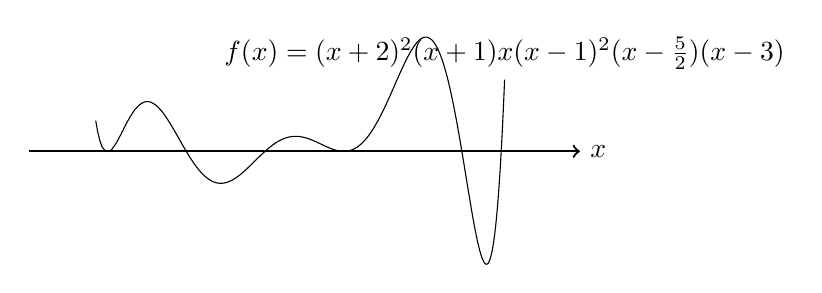
\begin{tikzpicture}
        % \draw[very thin,color=gray] (-0.1,-1.1) grid (3.9,8.1);
        \draw[->,thick] (-3,0) -- (4,0) node[right] {$x$}; 
        
        % \draw[domain=-6:6.5,samples=200] plot (\x,{sin((3*\x) r)});% node[right] {$f(x) = \sin x$};
        \draw[domain=-2.15:3.05,samples=500] plot (\x,{0.03*(\x+2)^2*(\x+1)*\x*(\x-1)^2*(\x-2.5)*(\x-3)}) node[above] {$f(x) = (x+2)^2(x+1)x(x-1)^2(x-\frac{5}{2})(x-3)$};
    \end{tikzpicture}
\end{center}

\end{enumerate}

\begin{formal}
    {\large \textbf{知识点三、含绝对值不等式的解法}}
\end{formal}

\begin{enumerate}
    \item 最简单的绝对值不等式的同解变形;
    $$
    |ax+b|<c \Leftrightarrow -c<ax+b<c 
    $$
    $$
    |ax+b|>c \Leftrightarrow ax+b<-c \text{\  或 \ }  ax+b>c
    $$
    \item 不等式$ |x|<a\ (a>0)$的解集就是求在数轴上到原点的距离小于$a$的点对应的实数$x$的集合.

\end{enumerate}
\clearpage
\section{第8课\quad 基本不等式及其应用}

\begin{formal}
    {\large \textbf{知识点一、平均值不等式}}
\end{formal}


\begin{enumerate}
    \item 对于正数$a,b$称$\displaystyle \frac{a+b}{2}\text{是}a,b\text{的算数平均值,并称}\sqrt{ab}\text{是}a,b\text{的几何平均值}$

    \item {\large{\textbf{平均值不等式:}}}\ 两个正数的算术平均值大于等于它们的几何平均值,即对于任意的正数,有
    $$
    \frac{a+b}{2}\ge \sqrt{ab},\ (a>0,b>0)
    $$
    当且仅当$a=b$是等号成立\\
    \\
    {\large{\textbf{三注意:}}}\\
    {\large{\textbf{“一正”:}}}不等式中的各项必须都是正数; \\
    {\large{\textbf{“二定”:}}}和定积最大,积定和最小; \\
    {\large{\textbf{“三相等”:}}}只有满足了不等式中等号成立的条件,才能使用基本不等式求最值.\\
    \item 平均值不等式的变式与推广
    \begin{enumerate}
        \item 加权平均$\ge$ 算术平均$\ge$ 几何平均:$\displaystyle \sqrt{\frac{a^2+b^2}{2}}\ge \frac{a+b}{2} \ge \sqrt{ab} , \ (a>0,b>0)$
    
        \item { 推广:$ a_1,a_2,a_3,\cdots,a_n$是$n$个正数,则$\displaystyle \frac{a_1,a_2,a_3,\cdots,a_n}{n}$称为这$n$个正数的算术平均数,
        $\sqrt[n]{a_1\cdot a_2\cdot a_3\cdot \cdots \cdot a_n}$称为这个正数的几何平均数,
        它们的关系是:$\displaystyle \frac{a_1,a_2,a_3,\cdots,a_n}{n} \ge \sqrt[n]{a_1\cdot a_2\cdot a_3\cdot \cdots \cdot a_n}$,当且仅当$  a_1=a_2=a_3=\cdots=a_n$时等号成立。}
    \end{enumerate}
\end{enumerate}


\begin{tcolorbox} 
题型一:基本不等式基本应用
\end{tcolorbox}
\par
\begin{problem}
    设$x>0$,证明$\displaystyle x+\frac{1}{x} \ge 2$,并指出等号成立条件
    \begin{jiexi}
        因为$x>0$,有平均值不等式得:
        $$x+\frac{1}{x} \ge 2\sqrt{x\cdot\frac{1}{x}} = 2$$
        当$x=\frac{1}{x}$,即$x=1$时等号成立.
    \end{jiexi}
\end{problem}

\par
\begin{problem}
    证明:若$ a<0$,则$\displaystyle a+\frac{1}{a} \le -2$,并指出等号成立条件。
    \begin{jiexi}
       根据题意,$a<0$,则$-a>0$,左式$\displaystyle =a+\frac{1}{a}=-[(-a)+(-\frac{1}{a})]$,\\
       又由$\displaystyle (-a)+(-\frac{1}{a})\ge 2\sqrt{(-a)\cdot(-\frac{1}{a})} = 2$,则有$a+\frac{1}{a}\le -2$,当且仅当$a=-1$时,等号成立
    \end{jiexi}
\end{problem}

\par
\begin{problem}
    $x \ne 0,x\in R,$,则$\displaystyle =x+\frac{1}{x}$的取值范围\tiankong{$(-\infty,-2]\cup[2,+\infty)$}
\end{problem}



\begin{tcolorbox} 
题型二:配凑法
\tcblower %增加了一条虚线
$$x+\frac{1}{x+a} \quad \Rightarrow \quad x+a+\frac{1}{x+a}-a$$
$$x(x-bx) \quad \Rightarrow \quad bx(a-bx)\cdot \frac{1}{b} $$
\end{tcolorbox}


\end{document}